% -*- latex -*-

This chapter documents the implementation and API of the Dax toolkit. This
documentation is primarily in reference to users of the Dax toolkit but
also gives some details on the internal implementation.

The Dax toolkit is written in C++ and makes extensive use of templates. The
toolkit is implemented as a header library, meaning that all the code is
implemented in header files (with extension \textfilename{.h}) and
completely included in any code that uses it. This is typically necessary
of template libraries, which need to be compiled with template parameters
that are not known until they are used. This also provides the convienience
of allowing the compiler to inline user code for better performance.

When documenting the Dax API, the following conventions are used.
\begin{itemize}
\item Filenames are printed in a \textfilename{sans serif font}.
\item C++ code is printed in a \textcode{monospace font}.
\item Macros and namespaces from the Dax toolkit are printed
  in \textnamespace{red}.
\item Identifiers from the Dax toolkit are printed in
  \textidentifier{blue}.
\item Signatures, described in Section~\ref{sec:GenericScheduling}, are
  printed in \textsignature{green}.
\end{itemize}

\section{Package Structure}
\label{sec:PackageStructure}

\index{packages|seealso{namespace}}
\index{packages|(}

The Dax toolkit is organized in a hierarchy of nested packages. The Dax
toolkit places definitions in \keyterm{namespaces} \index{namespace} that
correspond to the package (with the exception that one package may
specialized a template defined in a different namespace). Hence, the
description and

The base package is named \dax{}. All classes within the Dax toolkit are
placed either directly in the \dax{} package or in a package beneath
it. This helps prevent name collisions between the Dax toolkit and any
other library.

As described in Section~\ref{sec:StructureOfDaxFramework}, the Dax API is
divided into two distinct environments: \index{environments} the control
environment \index{control~environment} and the execution
environment. \index{execution~environment} The API for these two
environments are located in the \daxcont{} and \daxexec{} packages,
respectively. Items located in the base \dax{} namespace are available in
both environments.

Although it is conventional to spell out names in identifiers (see the
coding conventions in Section~\ref{sec:CodingConventions}), there is an
exception to abbreviate control and execution to \textnamespace{cont}
and \textnamespace{exec}, respectively. This is because it is also part of
the coding convention to declare the entire namespace when using an
identifier that is part of the corresponding package. The shorter names
make the identifiers easier to read, faster to type, and more feasible to
pack lines in 80 column displays. These abbreviations are also used instead
of more common abbreviations (e.g. ctrl for control) because, as part of
actual English words, they are easier to type.

Worklets provided by the Dax toolkit, described in
Section~\ref{sec:ProvidedWorklets}, are contained in the \daxworklet{}
package. Although the operation of a worklet happens exclusively in the
execution environment, worklets are typically initialized in the control
environment. Thus, the \daxworklet{} package is not encapsulated in either
\daxcont{} or \daxexec{}.

The Dax toolkit provides a base set of library functions that are ported to
the various systems and compilers on which it is used. These functions are
located in the \daxmath{} package. The features in \daxmath{} are available
in both the control and execution environments, but they are typically used
in the execution environment.

The Dax toolkit contains code that uses specalized compiler features, such
as those with CUDA and OpenMP, or libraries, such as Intel Threading
Building Blocks, that will not be available on all machines. Code for these
features are encapsulated in their own packages: \daxcuda{}, \daxopenmp{},
and \daxtbb{}. Within each one of these packages, there will
be \textnamespace{cont} and \textnamespace{exec} namespaces as necessary to
denote features that are accessible in only one environment or the other.

The Dax toolkit contains OpenGL interoperability \index{OpenGL}
\index{interoperability} that allows data generated with Dax to be
efficiently transfered to OpenGL objects. This feature is encapsulated in
the \daxopengl{} package.

Figure~\ref{fig:Packages} provides a diagram of the Dax package hierarchy.

\begin{figure}
  \centering
  %% \begin{itemizetight}
  %% \item \textnamespace{dax}
  %%   \begin{itemizetight}
  %%   \item \textnamespace{cont}
  %%   \item \textnamespace{exec}
  %%   \item \textnamespace{worklet}
  %%   \item \textnamespace{math}
  %%   \item \textnamespace{cuda}
  %%     \begin{itemizetight}
  %%     \item \textnamespace{cont}
  %%     \end{itemizetight}
  %%   \item \textnamespace{openmp}
  %%     \begin{itemizetight}
  %%     \item \textnamespace{cont}
  %%     \end{itemizetight}
  %%   \item \textnamespace{tbb}
  %%     \begin{itemizetight}
  %%     \item \textnamespace{cont}
  %%     \end{itemizetight}
  %%   \item \textnamespace{opengl}
  %%   \end{itemizetight}
  %% \end{itemizetight}
  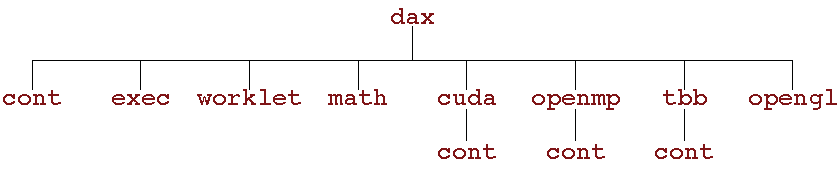
\includegraphics{images/PackageHierarchy}
  \caption{Dax package hierarchy.}
  \label{fig:Packages}
\end{figure}

By convention all classes will be defined in a file with the same name as
the class name (with a \textfilename{.h} extension) located in a directory
corresponding to the package name. For example, the \daxcont{ArrayHandle}
class is found in the \textfilename{dax/cont/ArrayHandle.h} header. There
are, however, exceptions to this rule. Some smaller classes and types are
grouped together for convienience. These exceptions will be noted as
necessary.

Within each namespace there may also be \textnamespace{internal}
\indexnamespaceone{internal} and \textnamespace{detail}
\indexnamespaceone{detail} sub-namespaces. The \textnamespace{internal}
namespaces contain features that are used internally and may change without
notice. The \textnamespace{detail} namespaces contain features that are
used by a particular class but must be declared outside of that
class. Users should generally ignore classes in these namespaces.

\index{packages|)}


\section{Basic Provisions}
\label{sec:BasicProvisions}

This section describes the core facilities provided by the Dax
toolkit. These include macros, types, and classes that define the
environment in which code is run, the core types of data stored, and
template introspection.

\subsection{Function and Method Exports}
\label{sec:FunctionAndMethodExports}

Any function or method defined by the Dax toolkit must come with an export
modifier that determines in which environments the function may be
run. These export modifiers are C macros that Dax uses to instruct the
compiler for which architectures to compile each method. Most user code
outside of the Dax toolkit need not use these macros with the important
exception of any classes passed to the Dax toolkit. This occurs when
defining new worklets, array containers, and device adapters.

Dax provides three export macros, \daxcontexport, \daxexecexport, and
\daxexeccontexport, which are used to declare functions and methods that
can run in the control environment, export environment, and both
environments, respectively. The export macro is place after the template
declaration, if there is one, and before the return type for the
function. Here is a simple example of a function that will square a
value. Since most types you would use this function on have operators in
both the control and execution environments, the function is exported to
both places.

\begin{lstlisting}
template<class ValueType>
DAX_EXEC_CONT_EXPORT
ValueType Square(const ValueType &inValue)
{
 return inValue * inValue;
}
\end{lstlisting}

The primary function of the export macros is to interject compiler-specific
keywords that specify what architecture to compile code for. For example,
when compiling with CUDA\index{CUDA}, the control exports have
\textcode{\_\_host\_\_} in them and execution exports have
\textcode{\_\_device\_\_} in them.

There is one additional export macro that is not used for functions but
rather used when declaring a constant data object that is used in the
execution environment. This macro is named
\textmacro{DAX\_EXEC\_CONSTANT\_EXPORT}\index{DAX\_EXEC\_CONSTANT\_EXPORT}\index{export!constant}\index{constant~export}
and is used to declare a constant lookup table used when executing a
worklet. Its primary reason for existing is to add a
\textcode{\_\_constant\_\_} keyword when compiling with CUDA. This export
currently has no effect on any other compiler.

\subsection{Core Data Types}
\label{sec:CoreDataTypes}

\fix{-dax::Id, dax::Scalar} \\
\fix{-dax::Id2, dax::Id3, dax::Vector2, dax::Vector3, dax::Vector4} \\
\fix{--Supported operators} \\
\fix{-dax::Tuple<>} \\
\fix{-dax::Pair<>}

\subsection{Traits}
\label{sec:Traits}

\fix{-type traits} \\
\fix{-vector traits} \\
\fix{-vector operations}


\section{Provided Worklets}
\label{sec:ProvidedWorklets}

\fix{Algorithm implementations provided by Dax.}

\fix{The tools provided to build new worklets, which is designed to be a
  simple process, are documented in
  Section~\ref{sec:ExecutionEnvironment}.}


\section{Control Environment}
\label{sec:ControlEnvironment}

\subsection{Device Adapter Tag}
\label{sec:DeviceAdapterTag}

\fix{Write}

\subsection{Array Handle}
\label{sec:ArrayHandle}

\fix{--Using} \\
\fix{--Interface to device} \\
\fix{---Prepare\textasteriskcentered} \\
\fix{--Containers} \\
\fix{---Basic} \\
\fix{---Adapting data structures} \\
\fix{---Implicit/derived} \\
\fix{---Transfer} \\

\subsection{Grid Structures}
\label{sec:GridStructures}

\fix{Uniform Grid, Unstructured Grid}

\subsection{Scheduling}
\label{sec:Scheduling}

\fix{Will the scheduler classes be changed in time?}

\subsection{Timers}
\label{sec:Timers}

\fix{Write}

\subsection{Error Handling}
\label{sec:ErrorHandling}

\fix{Write}

\subsection{Device Adapter Algorithms}
\label{sec:DeviceAdapterAlgorithms}

\subsubsection{Available Algorithms}

\fix{Write}

\subsubsection{Implementing Device Adapters}

\fix{Also talk about generic device adapter.}

\fix{What about implementing execution memory management?}


\section{Execution Environment}
\label{sec:ExecutionEnvironment}

\subsection{Creating Worklets}
\label{sec:CreatingWorklets}

\fix{-List of types}\\
\fix{-Base Classes}\\
\fix{-operator()} \\
\fix{-signatures} \\
\fix{-error handling}

\subsection{Math}
\label{sec:Math}

\fix{Portable math functions}

\subsection{Cells and Operations}

\fix{-tags} \\
\fix{-dax::exec::CellVertices} \\
\fix{-dax::exec::CellField} \\
\fix{-cell operations}


\section{OpenGL Interoperability}
\label{sec:OpenGLInteroperability}


\section{Coding Conventions}
\label{sec:CodingConventions}

\fix{-follows VTK conventions where possible}\\
\fix{-2 space indentation}\\
\fix{-no tabs}\\
\fix{-fit within 80 column display whenever possible}\\
\fix{-namespaces are lower case}\\
\fix{-Class names are camel case starting with upper case}\\
\fix{-Classes are declared in a file with the same name as the class in a
  directory corresponding to the package/namespace}\\
\fix{--Except where they're not}\\
\fix{-Method, function, and class field names are camel case starting with
  upper case}\\
\fix{--Except when conflicts with convention from some other library
  (e.g. make\_Vector2 corresponds to make\_pair in standard template
  library).}\\
\fix{-local variables and parameters are camel case starting with lower
  case}\\
\fix{-spelled out identifiers}\\
\fix{-specify full namespace when using classes}\\
\fix{-use this-> when referencing a class method or field}\\
